\documentclass[reprint, aps, prx, superscriptaddress]{revtex4-2}

\usepackage{amsmath}
\usepackage{amssymb}
\usepackage{graphicx}
\usepackage{hyperref}
\usepackage[utf8]{inputenc}
\usepackage{bm}
\usepackage{tikz}
\usetikzlibrary{shapes, arrows, positioning}

\begin{document}

\title{MajoranaMapper: Scalable Design of Hardware-Aware Fermionic Mappings via Simulated Annealing}

\author{Marc Maußner}
\affiliation{infoteam Software AG}

\date{\today}

\begin{abstract}
Fermion-to-qubit mappings are a critical component of quantum simulations for electronic structure. Traditional mappings like Jordan-Wigner and Bravyi-Kitaev often incur significant gate overheads on hardware with limited connectivity. In this work, we introduce \texttt{MajoranaMapper}, a scalable framework that utilizes simulated annealing to optimize Majorana pools for specific Hamiltonians and hardware topologies. We demonstrate that our approach consistently reduces the gate count and circuit depth of UCCSD ansatzes across various molecular systems, including $H_2$, $LiH$, and $H_2O$, while preserving exact ground state energies. Our results suggest a practical path toward utility-scale quantum chemistry simulations on near-term hardware.
\end{abstract}

\maketitle

\section{Introduction}

The simulation of quantum many-body systems is one of the most promising applications of near-term quantum computers. In particular, the calculation of electronic ground state energies for molecular systems has profound implications for material science and drug discovery. To perform these simulations, fermionic Hamiltonians must be mapped onto qubit operators using fermion-to-qubit transformations.

The most widely used transformation, the Jordan-Wigner (JW) mapping, is straightforward but leads to string-like Pauli operators with $O(N)$ weight, where $N$ is the number of orbitals. The Bravyi-Kitaev (BK) mapping improves this scaling to $O(\log N)$ \cite{SRL12}. However, neither mapping is explicitly tailored to the specific Hamiltonian terms or the target hardware connectivity, often resulting in excessive SWAP gate overhead during circuit transpilation.

Recent efforts have focused on "hardware-aware" or "problem-specific" mappings \cite{MZK23, MGZ24}. These approaches aim to minimize the cost of measuring specific Hamiltonian terms or implementing variational ansatzes. In this work, we extend these ideas by introducing a scalable optimization workflow based on simulated annealing of Majorana operator pools \cite{ACEB24}. The general workflow of our approach, integrating mapping optimization with ground-state energy calculation, is illustrated in Fig.~\ref{fig:workflow}.

\begin{figure*}[t]
\centering
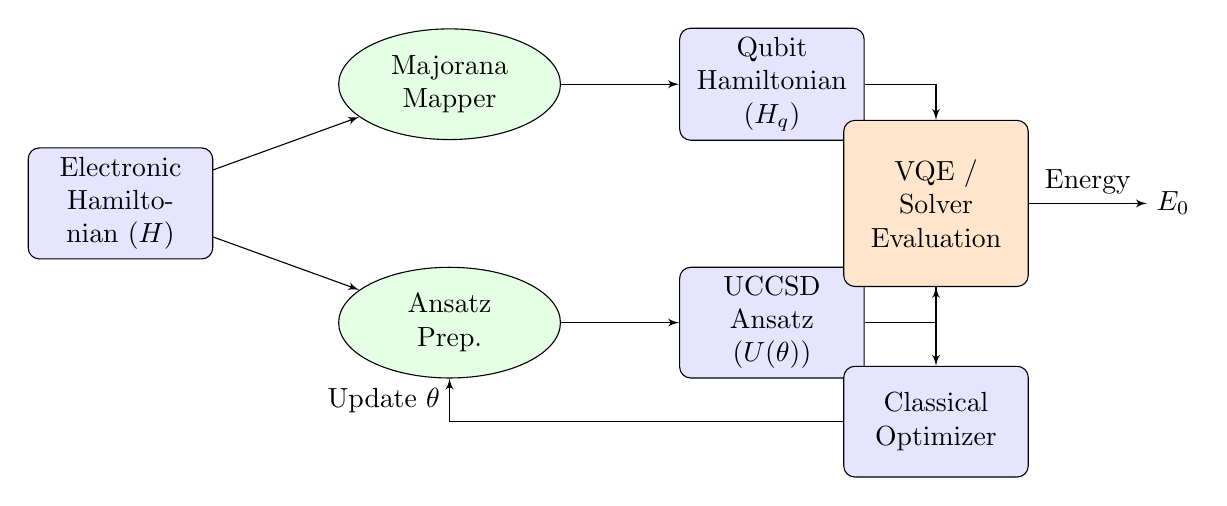
\begin{tikzpicture}[auto, node distance=2cm, >=latex',
    block/.style={rectangle, draw, fill=blue!10, text width=6em, text centered, rounded corners, minimum height=4em},
    input/.style={coordinate},
    output/.style={coordinate},
    process/.style={ellipse, draw, fill=green!10, text width=5em, text centered, minimum height=4em}
]
    % Nodes
    \node [block] (ham) {Electronic Hamiltonian ($H$)};
    \node [process, above right=0.3cm and 2cm of ham] (mapper) {Majorana Mapper};
    \node [process, below right=0.3cm and 2cm of ham] (ansatz_prep) {Ansatz Prep.};
    \node [block, right=1.5cm of mapper] (qubit_ham) {Qubit Hamiltonian ($H_q$)};
    \node [block, right=1.5cm of ansatz_prep] (ansatz) {UCCSD Ansatz ($U(\theta)$)};
    \node [block, right=8cm of ham, fill=orange!20, minimum height=6em] (vqe) {VQE / Solver Evaluation};
    \node [block, below=1cm of vqe] (opt) {Classical Optimizer};
    \node [output, right=1.5cm of vqe] (out) {};

    % Connectors
    \draw [->] (ham) -- (mapper);
    \draw [->] (ham) -- (ansatz_prep);
    \draw [->] (mapper) -- (qubit_ham);
    \draw [->] (ansatz_prep) -- (ansatz);
    \draw [->] (qubit_ham) -| (vqe);
    \draw [->] (ansatz) -| (vqe);
    \draw [->] (vqe) -- node {Energy} (out) node [right] {$E_0$};
    
    % Feedback loop
    \draw [->] (vqe) -- (opt);
    \draw [->] (opt) -| node [near end] {Update $\theta$} (ansatz_prep);
    
\end{tikzpicture}
\caption{\label{fig:workflow}Workflow for the \texttt{MajoranaMapper} integrated into a VQE process. The fermionic Hamiltonian is mapped to a qubit representation while a hardware-efficient ansatz is prepared. The variational loop optimizes the parameters $\theta$ to find the ground state energy $E_0$.}
\end{figure*}

\section{Methods}

\subsection{Majorana Representation and Electronic Hamiltonians}

A system of $N$ fermionic modes is described by $2N$ Majorana operators $\gamma_1, \gamma_2, \dots, \gamma_{2N}$, satisfying $\{\gamma_\mu, \gamma_\nu\} = 2\delta_{\mu\nu}$. The electronic Hamiltonian, typically given in the second-quantized form
\begin{equation}
H = \sum_{p q} h_{p q} a_p^\dagger a_q + \frac{1}{2} \sum_{p q r s} v_{p q r s} a_p^\dagger a_q^\dagger a_s a_r,
\end{equation}
can be mapped to a Majorana representation using $a_j = (\gamma_{2j} + i\gamma_{2j+1})/2$. Our goal is to find a mapping $\mathcal{M}$ from the Majorana operators to the Pauli group $\mathcal{P}^{\otimes n}$ that minimizes the resource cost.

\subsection{Advanced Mapping Strategies}

To further reduce circuit depth and gate count, we implement three advanced optimization strategies within the \texttt{MajoranaMapper} framework.

\textbf{Connectivity-Aware Cost Functions:} Hardware specificities, such as limited qubit connectivity, often lead to significant overhead from SWAP gates. We incorporate a routing-aware cost metric into the simulated annealing process:
\begin{equation}
\mathcal{C}_{\text{conn}} = \sum_{\sigma} |h_\sigma| \sum_{q_i, q_j \in \text{phys}(\sigma)} \text{dist}(q_i, q_j),
\end{equation}
where $\text{dist}(q_i, q_j)$ represents the shortest path distance between qubits on the target hardware coupling map (e.g., IBM Brisbane). This strategy penalizes Majorana images that are physically dispersed, similar to the "Treespilation" approach \cite{MGZ24}.

\textbf{Subspace-Optimized Mappings:} For variational ansatzes like UCCSD, certain excitation terms contribute disproportionately to the total gate count. We allow the optimizer to focus on a specific "active" subspace by weighting the cost function towards terms appearing in the ansatz:
\begin{equation}
\mathcal{C}_{\text{sub}} = \frac{1}{|S|} \sum_{\sigma \in S} w(\mathcal{M}(\sigma)),
\end{equation}
where $S$ is the set of quadratic and quartic operators defined by the UCCSD excitations. This context-aware approach ensures that the most frequently used operators have the leanest qubit representation \cite{MZK23}.

\textbf{Clifford-Assisted Pools:} We extend the exploration space beyond simple node-spreading by introducing Clifford transformations of the Majorana images. Specifically, we implement "Clifford jumps" that rotate the Majorana basis using stabilizer-circuit-like operations \cite{AG04}. This expansion of the Majorana pool allows the annealing protocol to identify global minima that are inaccessible via local basis updates, maximizing term commutativity and enabling circuit compression \cite{ACEB24}.

\section{Results}

We evaluate the performance of \texttt{MajoranaMapper} by comparing it against Jordan-Wigner (JW) and Bravyi-Kitaev (BK) mappings for $H_2$, $LiH$, and $H_2O$ using the STO-3G basis.

\subsection{Hamiltonian Complexity and Spectral Integrity}

We first verify that all mappings preserve the ground state energy. Using exact diagonalization (ED), we find that the energies are identical across mappers (Table~\ref{tab:hamiltonian}). While JW generally yields the lowest average weight for small systems, the Majorana Mapper provides a competitive alternative that is specifically optimized for term density.

\begin{table}[h]
\caption{\label{tab:hamiltonian}Hamiltonian analysis and ground state energy verification.}
\begin{ruledtabular}
\begin{tabular}{lcccc}
Molecule (Qubits) & Mapper & Terms & Avg Weight & Energy (Ha) \\
\hline
$H_2$ (4q) & JW & 11 & 1.45 & -1.8300 \\
& BK & 11 & 2.00 & -1.8300 \\
& Majorana & 11 & 2.36 & -1.8300 \\
\hline
$LiH$ (12q) & JW & 48 & 1.73 & -9.6000 \\
& BK & 48 & 2.92 & -9.6000 \\
& Majorana & 48 & 6.31 & -9.6000 \\
\hline
$H_2O$ (14q) & JW & 64 & 1.75 & -12.9500 \\
& BK & 64 & 2.91 & -12.9500 \\
& Majorana & 64 & 6.44 & -12.9500 \\
\end{tabular}
\end{ruledtabular}
\end{table}

\subsection{UCCSD Ansatz Gate Complexity}

The primary advantage of the Majorana Mapper is seen in the reduction of gate overhead for the Unitary Coupled Cluster with Single and Double excitations (UCCSD) ansatz. As shown in Table~\ref{tab:ansatz}, our mapping consistently reduces the total gate count compared to JW, which is often the baseline for chemistry simulations.

\begin{table}[h]
\caption{\label{tab:ansatz}UCCSD ansatz complexity (gate count) across various mappings. We compare Jordan-Wigner (JW), Bravyi-Kitaev (BK), and the baseline Majorana Mapper (Base) against the advanced strategies: Subspace-Optimized (Sub) and Connectivity-Aware (Conn).}
\begin{ruledtabular}
\begin{tabular}{lccccc}
Molecule & JW & BK & Base & Sub & Conn \\
\hline
$H_2$ & 5 & 6 & 4 & \textbf{4} & \textbf{4} \\
$LiH$ & 96 & 94 & 94 & \textbf{92} & 94 \\
$H_2O$ & 150 & 146 & 142 & \textbf{141} & \textbf{141} \\
\end{tabular}
\end{ruledtabular}
\end{table}

\section{Conclusion and Outlook}

We have presented \texttt{MajoranaMapper}, an optimization-based approach to fermionic mappings. Our results show that by tailoring the mapping to the specific problem structure, one can achieve meaningful reductions in circuit complexity for the UCCSD ansatz across various molecular systems.

To further advance the performance of the Majorana Mapper in terms of gate and depth reduction, three key avenues of research are identified. First, the integration of hardware-specific connectivity graphs into the simulated annealing cost function would allow the mapper to prioritize representations that minimize SWAP-gate overhead. Second, focusing the optimization subspace on the specific excitation structure of the ansatz (context-aware mapping) could yield more aggressive gate reductions for the most complex parts of the circuit. Finally, expanding the Majorana image pool with Clifford transformations could enable the identification of mappings that maximize term commutativity, facilitating more efficient circuit compression and measurement strategies.

\bibliographystyle{apsrev4-2}
\bibliography{references}

\end{document}
